\documentclass{beamer}
\usepackage{beamerthemesplit} 
\usepackage[utf8]{inputenc}
\usepackage{default}
\usepackage{graphicx}
\usepackage{float}
\usepackage{color, colortbl}
\usepackage{xcolor}
\usepackage{caption}
\usepackage{subcaption}
\usepackage{threeparttable}
\usepackage{amsmath}


\title{Localization Procedure}
	\subtitle{Orchestrating position estimation protocols in randomly deployed WSNs}
\author[Sanabria-Russo. L, Cano. C, Bellalta. B.]{Luis Sanabria-Russo, Cristina Cano, Boris Bellalta}
\institute[UPF]{Universitat Pompeu Fabra\\
				NeTS Research Group\\
				Barcelona, Spain}
\date{\today}



\begin{document}
%------------------Title Page---------------------%
\frame{\titlepage}

%\frame{\frametitle{Table of contents}\tableofcontents}

\section{Introduction}\label{intro}
\frame{\frametitle{What are Randomly Deployed WSNs?}
	\begin{itemize}
		\item Nodes are placed randomly over a field.
		\item It also encompasses deployments made at convenience (like home surveillance).
	\end{itemize}
	
	\begin{figure}[htbp]
		\centering
		\begin{subfigure}{.5\textwidth}
			\centering
			\includegraphics[width=0.565\linewidth, angle=-90]{figures/topology.eps}
			\caption{\tiny Example random deployment of nodes
			\label{fig:topology}}
			\end{subfigure}%
		\begin{subfigure}{.5\textwidth}
			\centering
			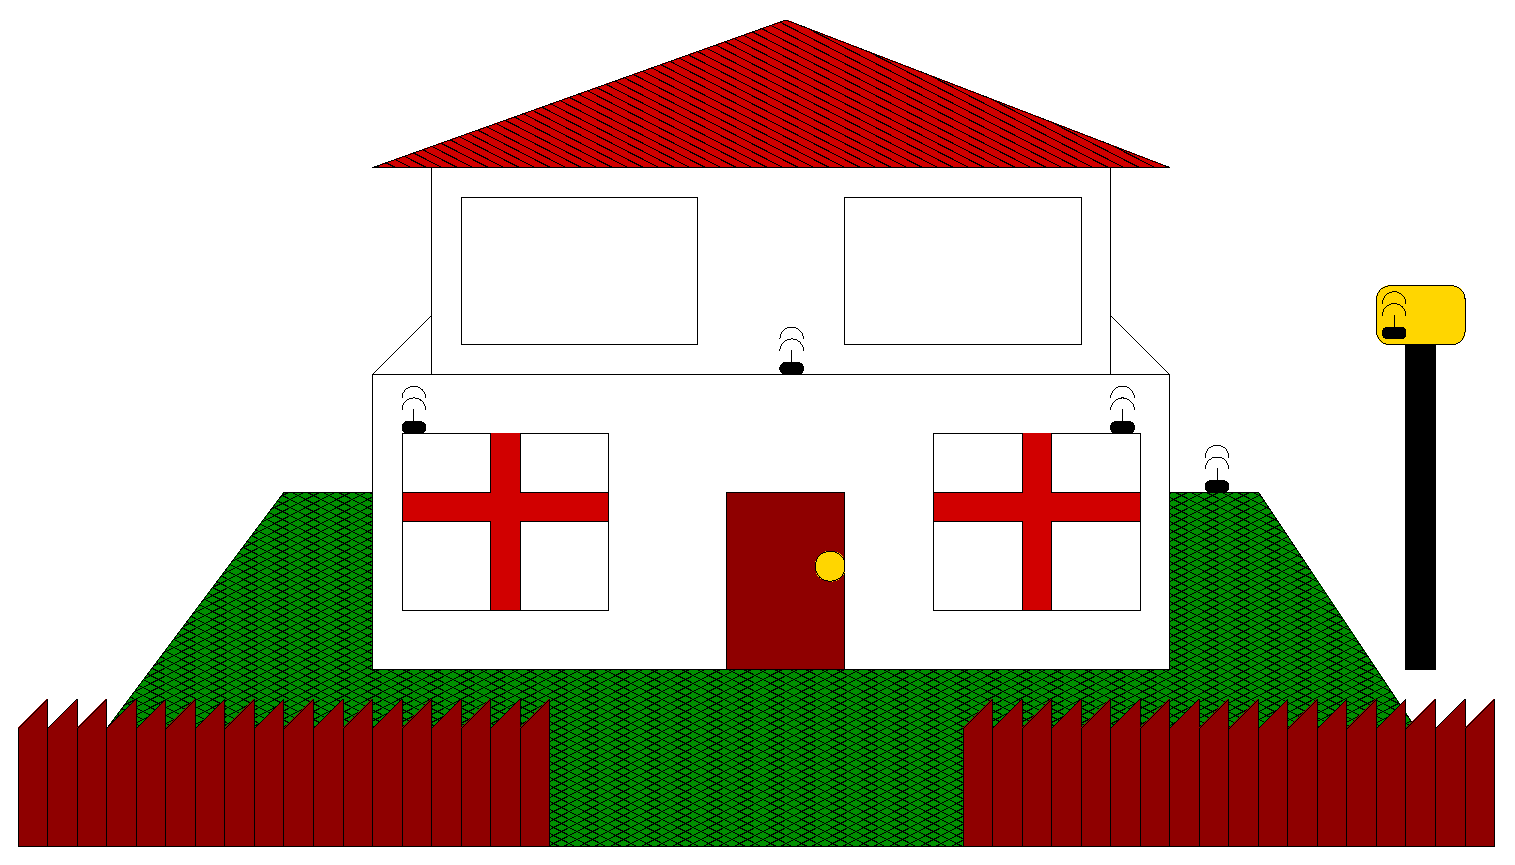
\includegraphics[width=\linewidth]{figures/house.eps}
			\caption{\tiny Example home surveillance deployment
			\label{fig:house}}
			\end{subfigure}
%	\caption{}
	\end{figure}
}


	\subsection{Characteristics}
	\frame{\frametitle{Characteristics}
		\begin{itemize}
			\item Nodes determine the best route to the sink.
			\item Collected metrics are back-traceable to its place of origin.
			\item In case of a battery run-out, nodes can be easily replaced.
		\end{itemize}
		
		\begin{figure}
			\centering
			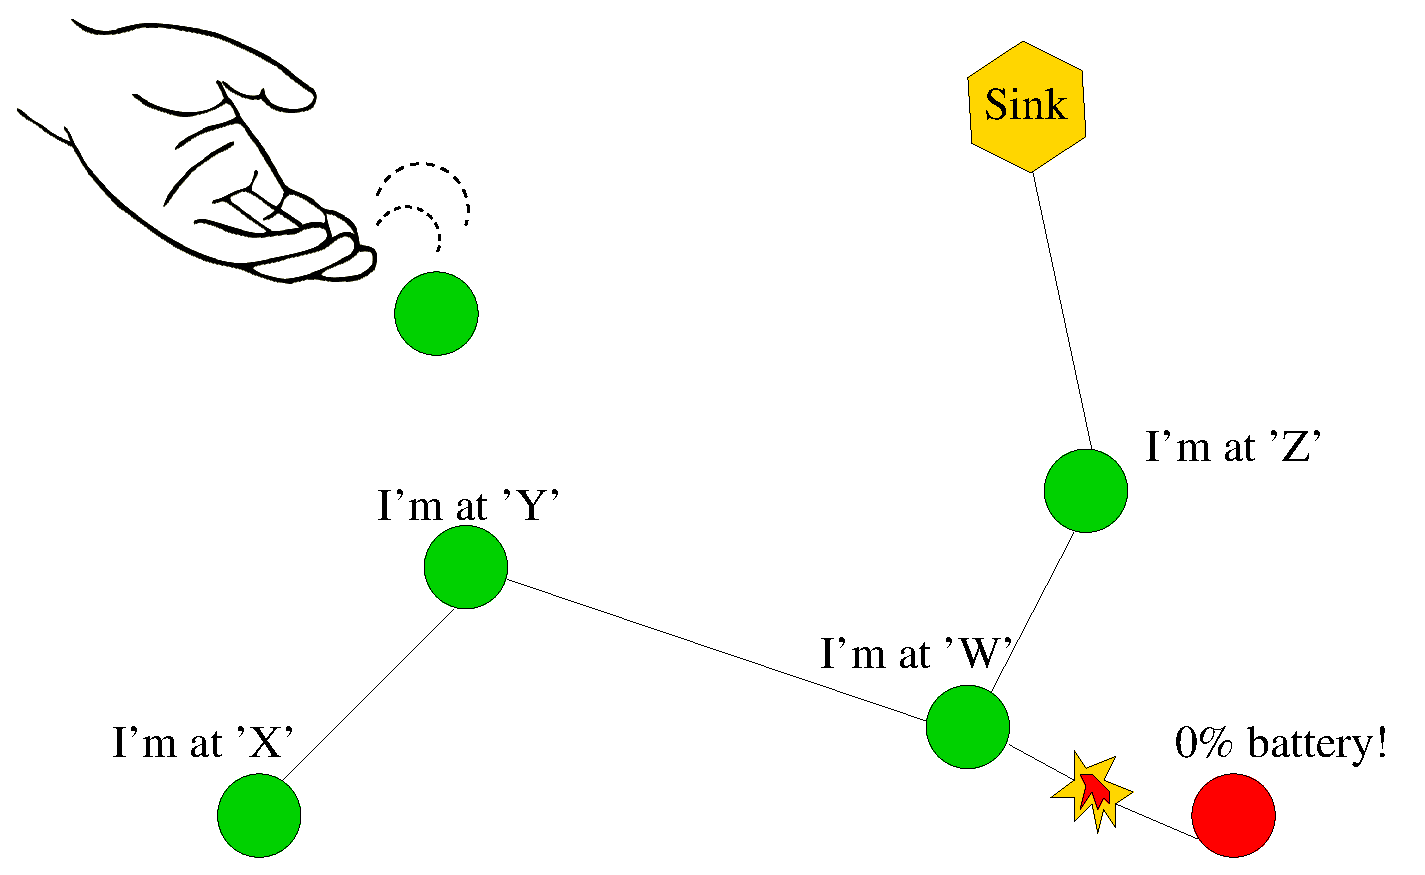
\includegraphics[width=0.565\linewidth]{figures/replacement.eps}
			\caption{\tiny Replacing nodes
			\label{fig:replacement}}
		\end{figure}%
	}

	
	\subsection{Applications}
	\frame{\frametitle{Applications}
		Because of their ease of deployment, randomly deployed WSNs are often used for:
			\begin{itemize}
				\item Volcano activity monitoring.
				\begin{itemize}
					\item Very dangerous or difficult places for deployment.
				\end{itemize}
				\item Forest fire detection.
				\begin{itemize}
					\item Very big areas.
				\end{itemize}
			\end{itemize}
		\begin{figure}
			\centering
			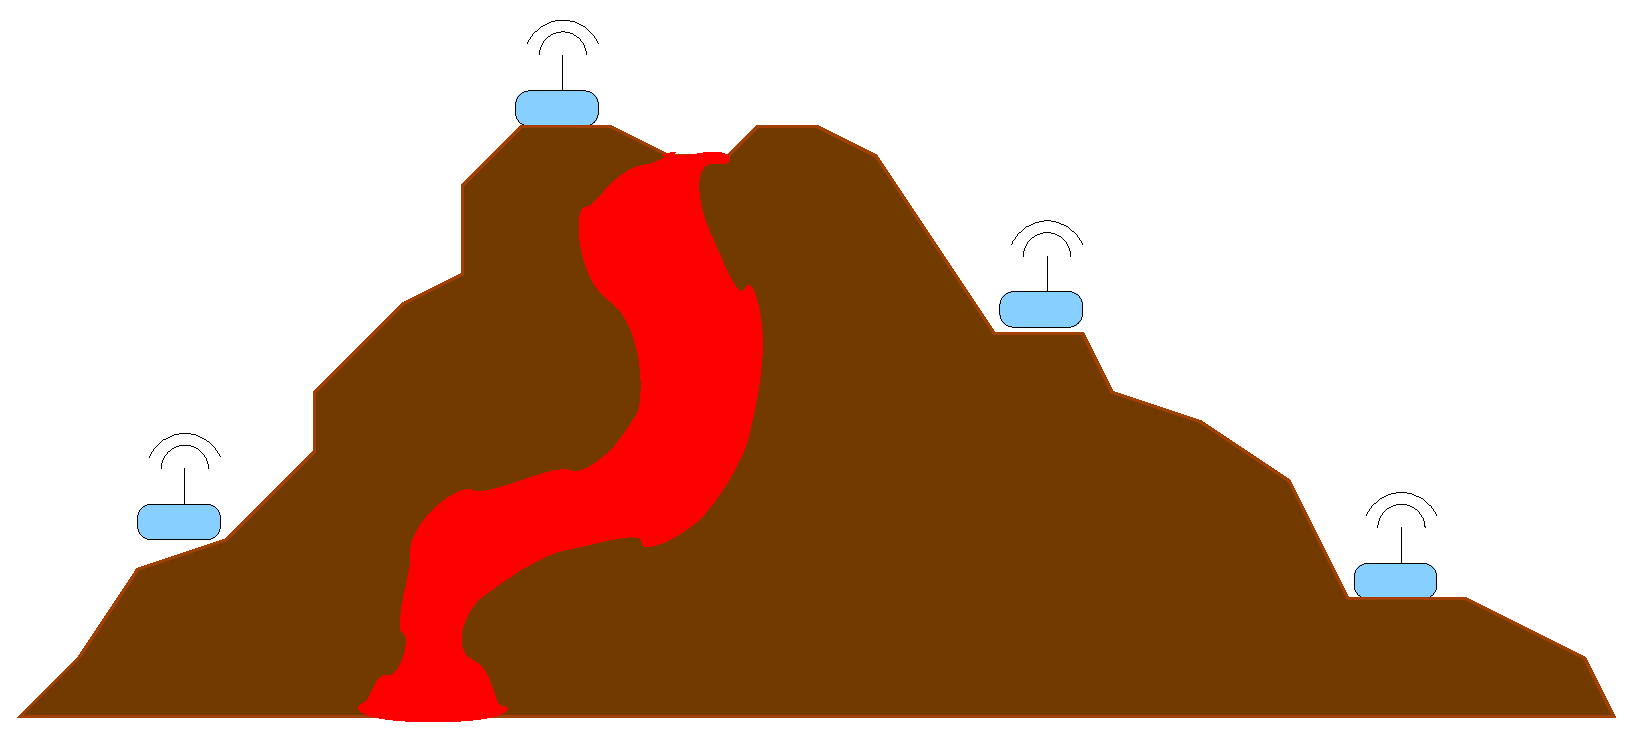
\includegraphics[width=0.565\linewidth]{figures/volcano.eps}
			\caption{\tiny Volcano monitoring example
			\label{fig:volcano}}
		\end{figure}%
	}
	
	\subsection{Pro's and Con's}
	\frame{\frametitle{Pro's and Con's of random deployments}
	Pro's:
	\begin{itemize}
		\item Allows rapid deployment.
		\item Reach very restrictive or dangerous places.
		\item Allows fast network reinforcement.
	\end{itemize}
	
	Con's:
	\begin{itemize}
		\item Metrics need to be traceable to their origin.
		\item Relies on location aware nodes (\emph{Anchors}).
		\item Localization often decreases network lifetime.
	\end{itemize}
	}
	
\section{Node Localization}
\frame{\frametitle{Node Localization}
	To make metrics traceable:
	\begin{enumerate}
		\item All nodes are equipped with GPS modules.
		\begin{enumerate}
			\item Decreasing network lifetime due to the modules~$\color{red}\downarrow$.
			\item Increasing the size and weight of the nodes~$\color{red}\downarrow$.
			\item Augmenting the required budget~$\color{red}\downarrow$.
			\item Very low estimation error~$\color{green}\uparrow$.
		\end{enumerate}
		\item Some nodes use GPS modules
		\begin{enumerate}
			\item Nodes derive a position estimation from Anchors: increased estimation error~$\color{red}\downarrow$.
			\item Additional workload is added to the nodes (estimation)~$\color{red}\downarrow$.
			\item Added network traffic (\emph{Beacons}) containing location information~$\color{red}\downarrow$.
			\item Cheaper and scalable approach~$\color{green}\uparrow$.
		\end{enumerate}
	\end{enumerate}
}

	\subsection{Measuring Distances}
	\frame{\frametitle{Measuring Distances}
		\begin{itemize}
			\item Any \emph{Unknown} node (unaware of its position) may derive an estimation from Beacons.
			\item Beacons are packets containing the position of the sender (usually an Anchor).
		\end{itemize}
		\begin{figure}[htbp]
			\centering
			\begin{subfigure}{.5\textwidth}
				\centering
				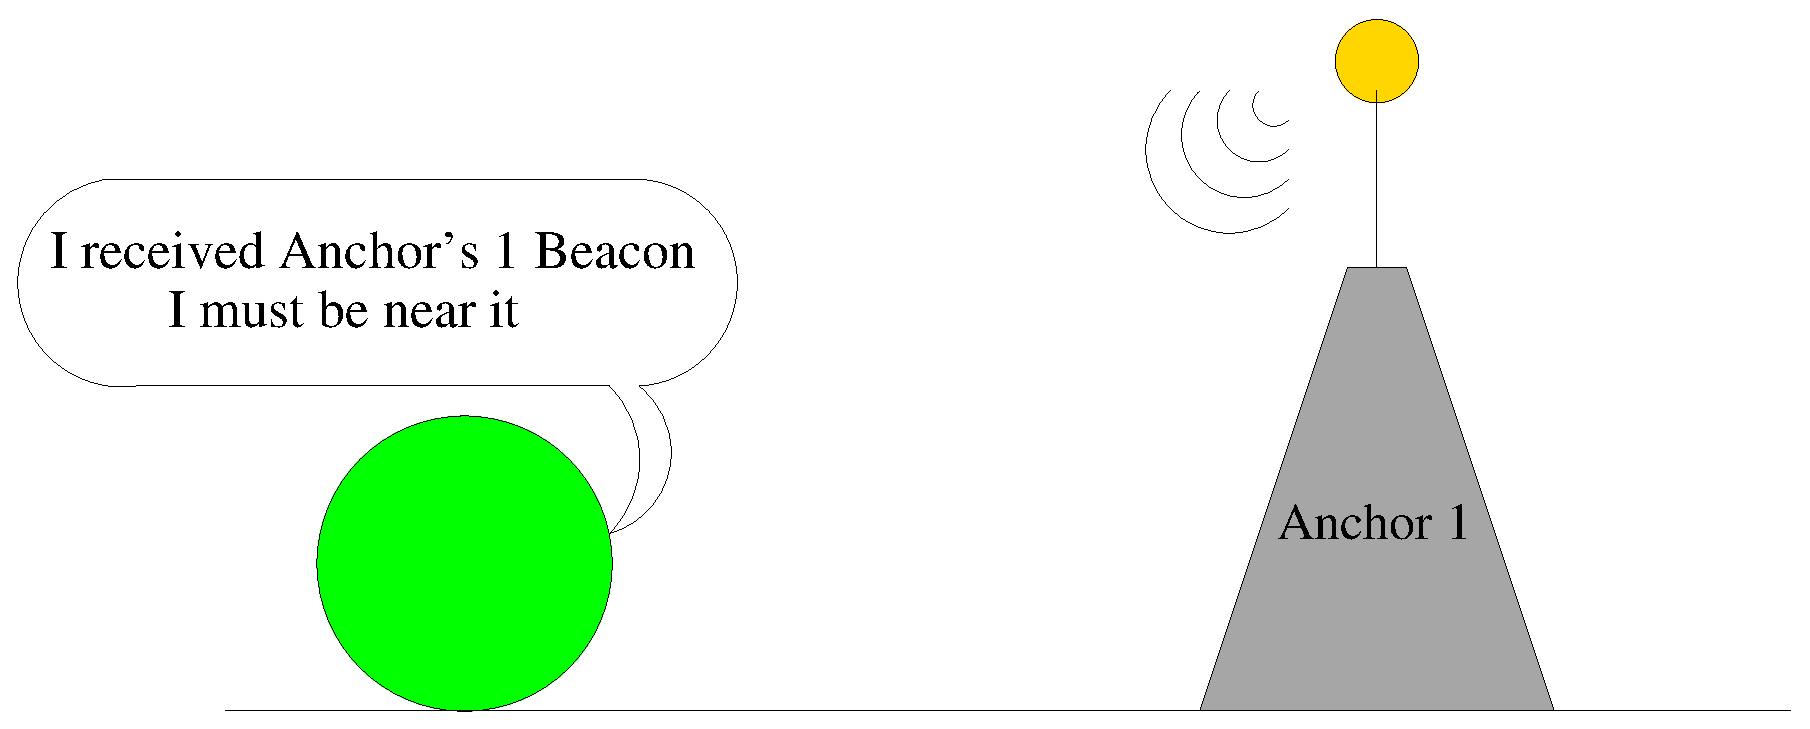
\includegraphics[width=\linewidth]{figures/coverage1.eps}
				\caption{\tiny Estimating a position with 1 Beacon
				\label{fig:coverage1}}
			\end{subfigure}%
			\begin{subfigure}{.5\textwidth}
				\centering
				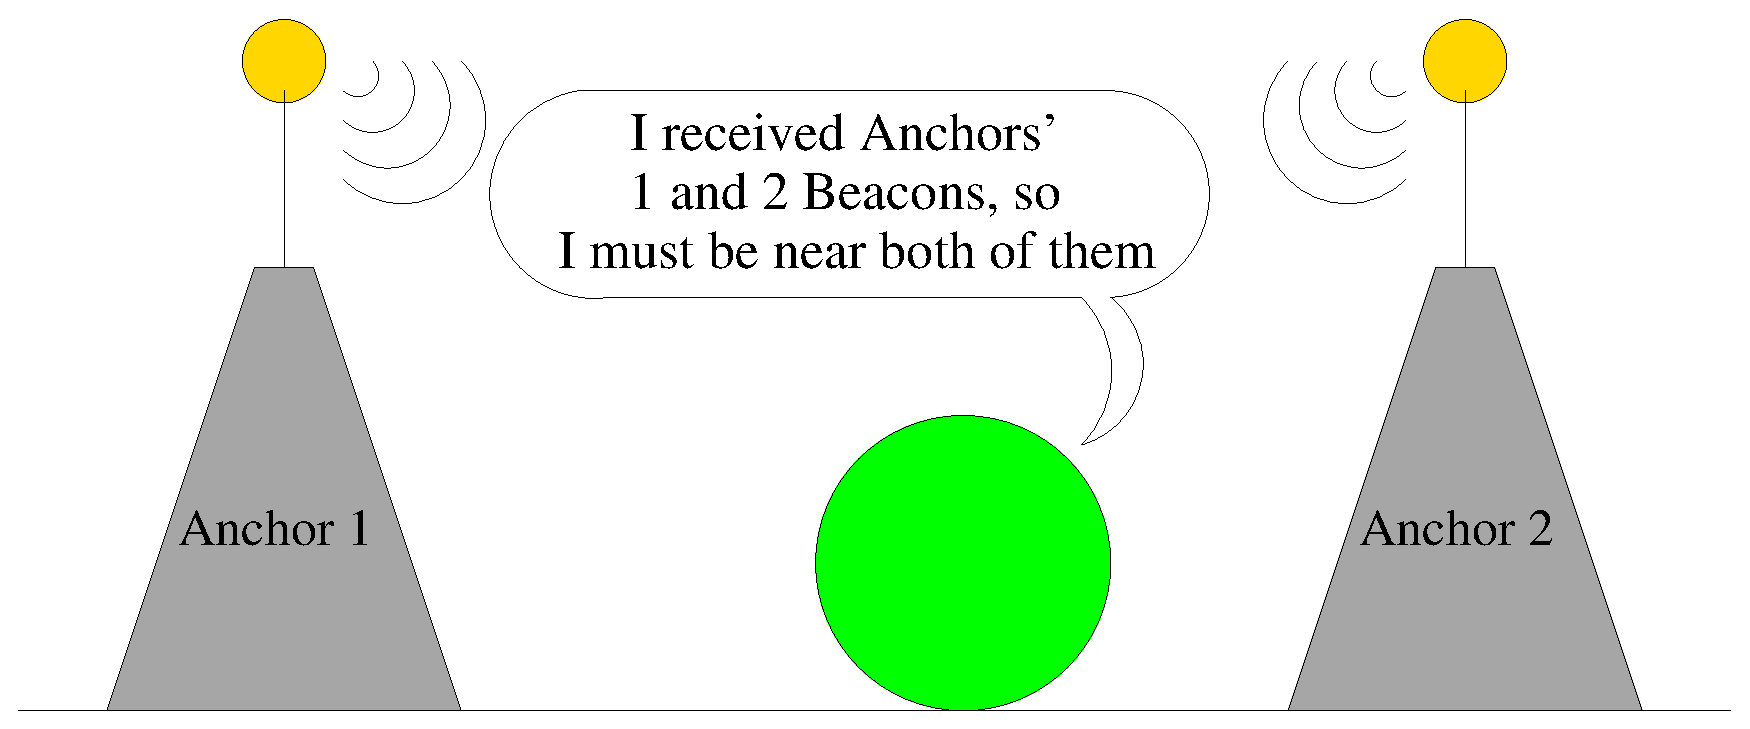
\includegraphics[width=0.97\linewidth]{figures/coverage2.eps}
				\caption{\tiny Estimating a position with 2 Beacons
				\label{fig:converage2}}
			\end{subfigure}
		%	\caption{}
		\end{figure}
		\begin{itemize}
			\item Applications may tolerate different levels estimation errors.
		\end{itemize}
	}
	
	\frame{\frametitle{Making Range Estimations}
		\begin{itemize}
		 \item Make use of the electromagnetic characteristics of the Beacon transmissions to derive a straight line estimation to the transmitter.
		\end{itemize}
		\begin{figure}[htbp]
			\centering
			\begin{subfigure}{.5\textwidth}
				\centering
				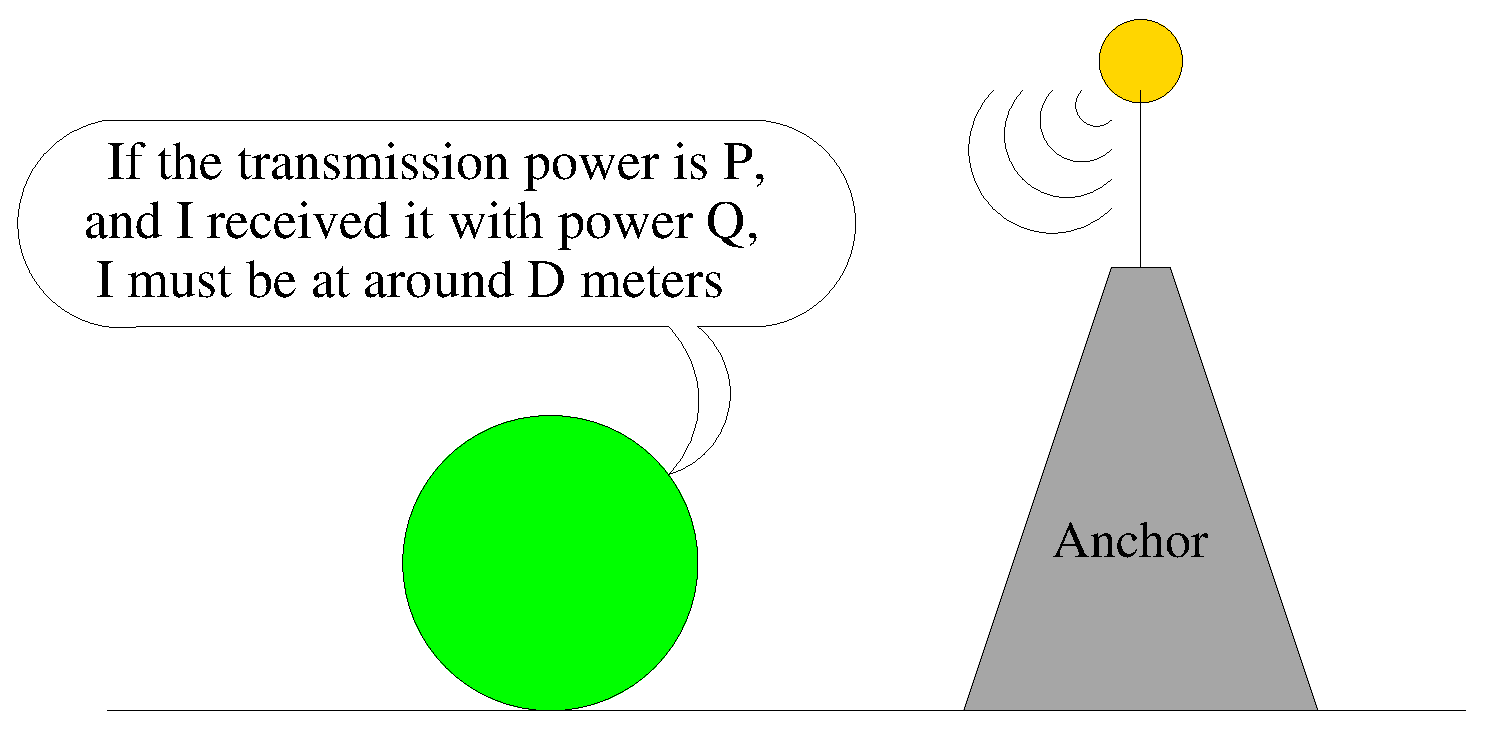
\includegraphics[width=\linewidth]{figures/RSSI.eps}
				\caption{\tiny RSSI position estimation
				\label{fig:RSSI}}
			\end{subfigure}%
			\begin{subfigure}{.5\textwidth}
				\centering
				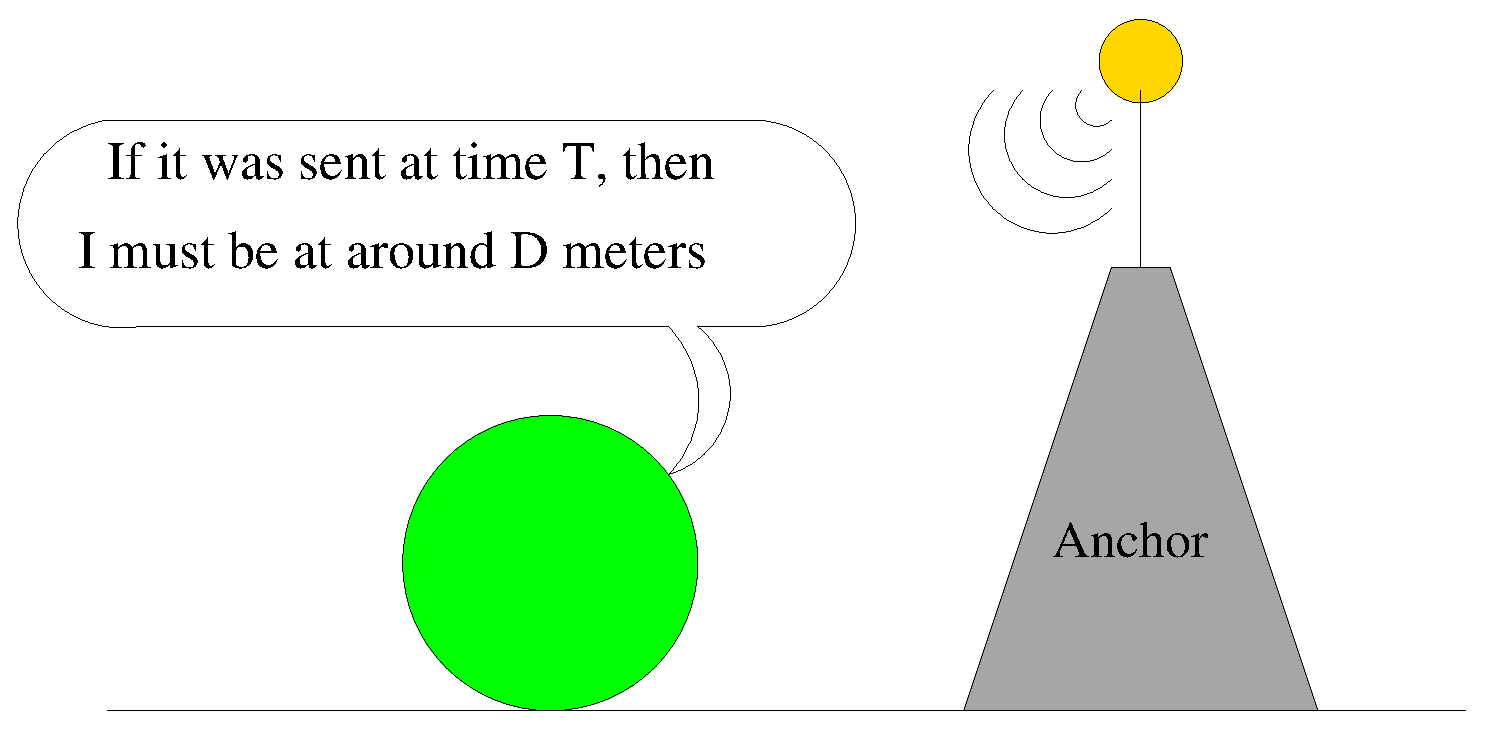
\includegraphics[width=\linewidth]{figures/ToA.eps}
				\caption{\tiny Time of Arrival (ToA)
				\label{fig:ToA}}
			\end{subfigure}
		%	\caption{}
		\end{figure}
	}
	
	\subsection{Localization Protocols}
	\frame{\frametitle{Localization Protocols}
		%In \emph{Anchor-based} deployments, position estimation protocols are often divided in:\\
		\begin{minipage}[l]{0.5\textwidth}
			{\bfseries ~~~~~~~~~~~~~Range-free}
			\begin{figure}
				\centering
				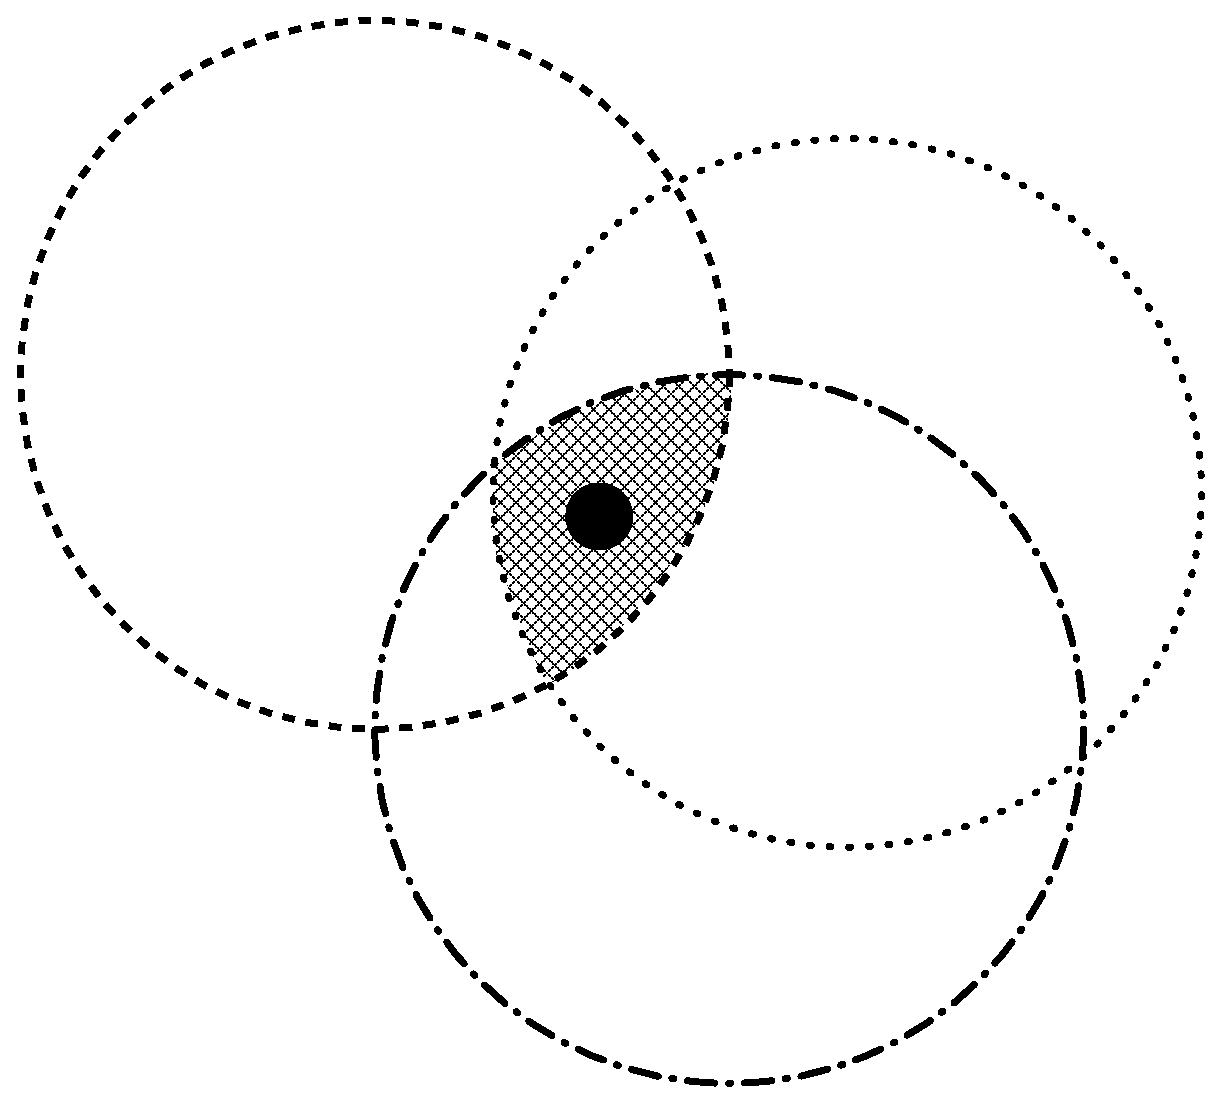
\includegraphics[width=0.75\linewidth]{figures/bounding_box.eps}
				\caption{\small Bounding-Box example
				\label{fig:bounding-box}}
			\end{figure}%

		\end{minipage}%
		\hfill
		\begin{minipage}[r]{0.5\textwidth}
			{\bfseries ~~~~~~~~~~Range-based}
			\begin{figure}
				\centering
				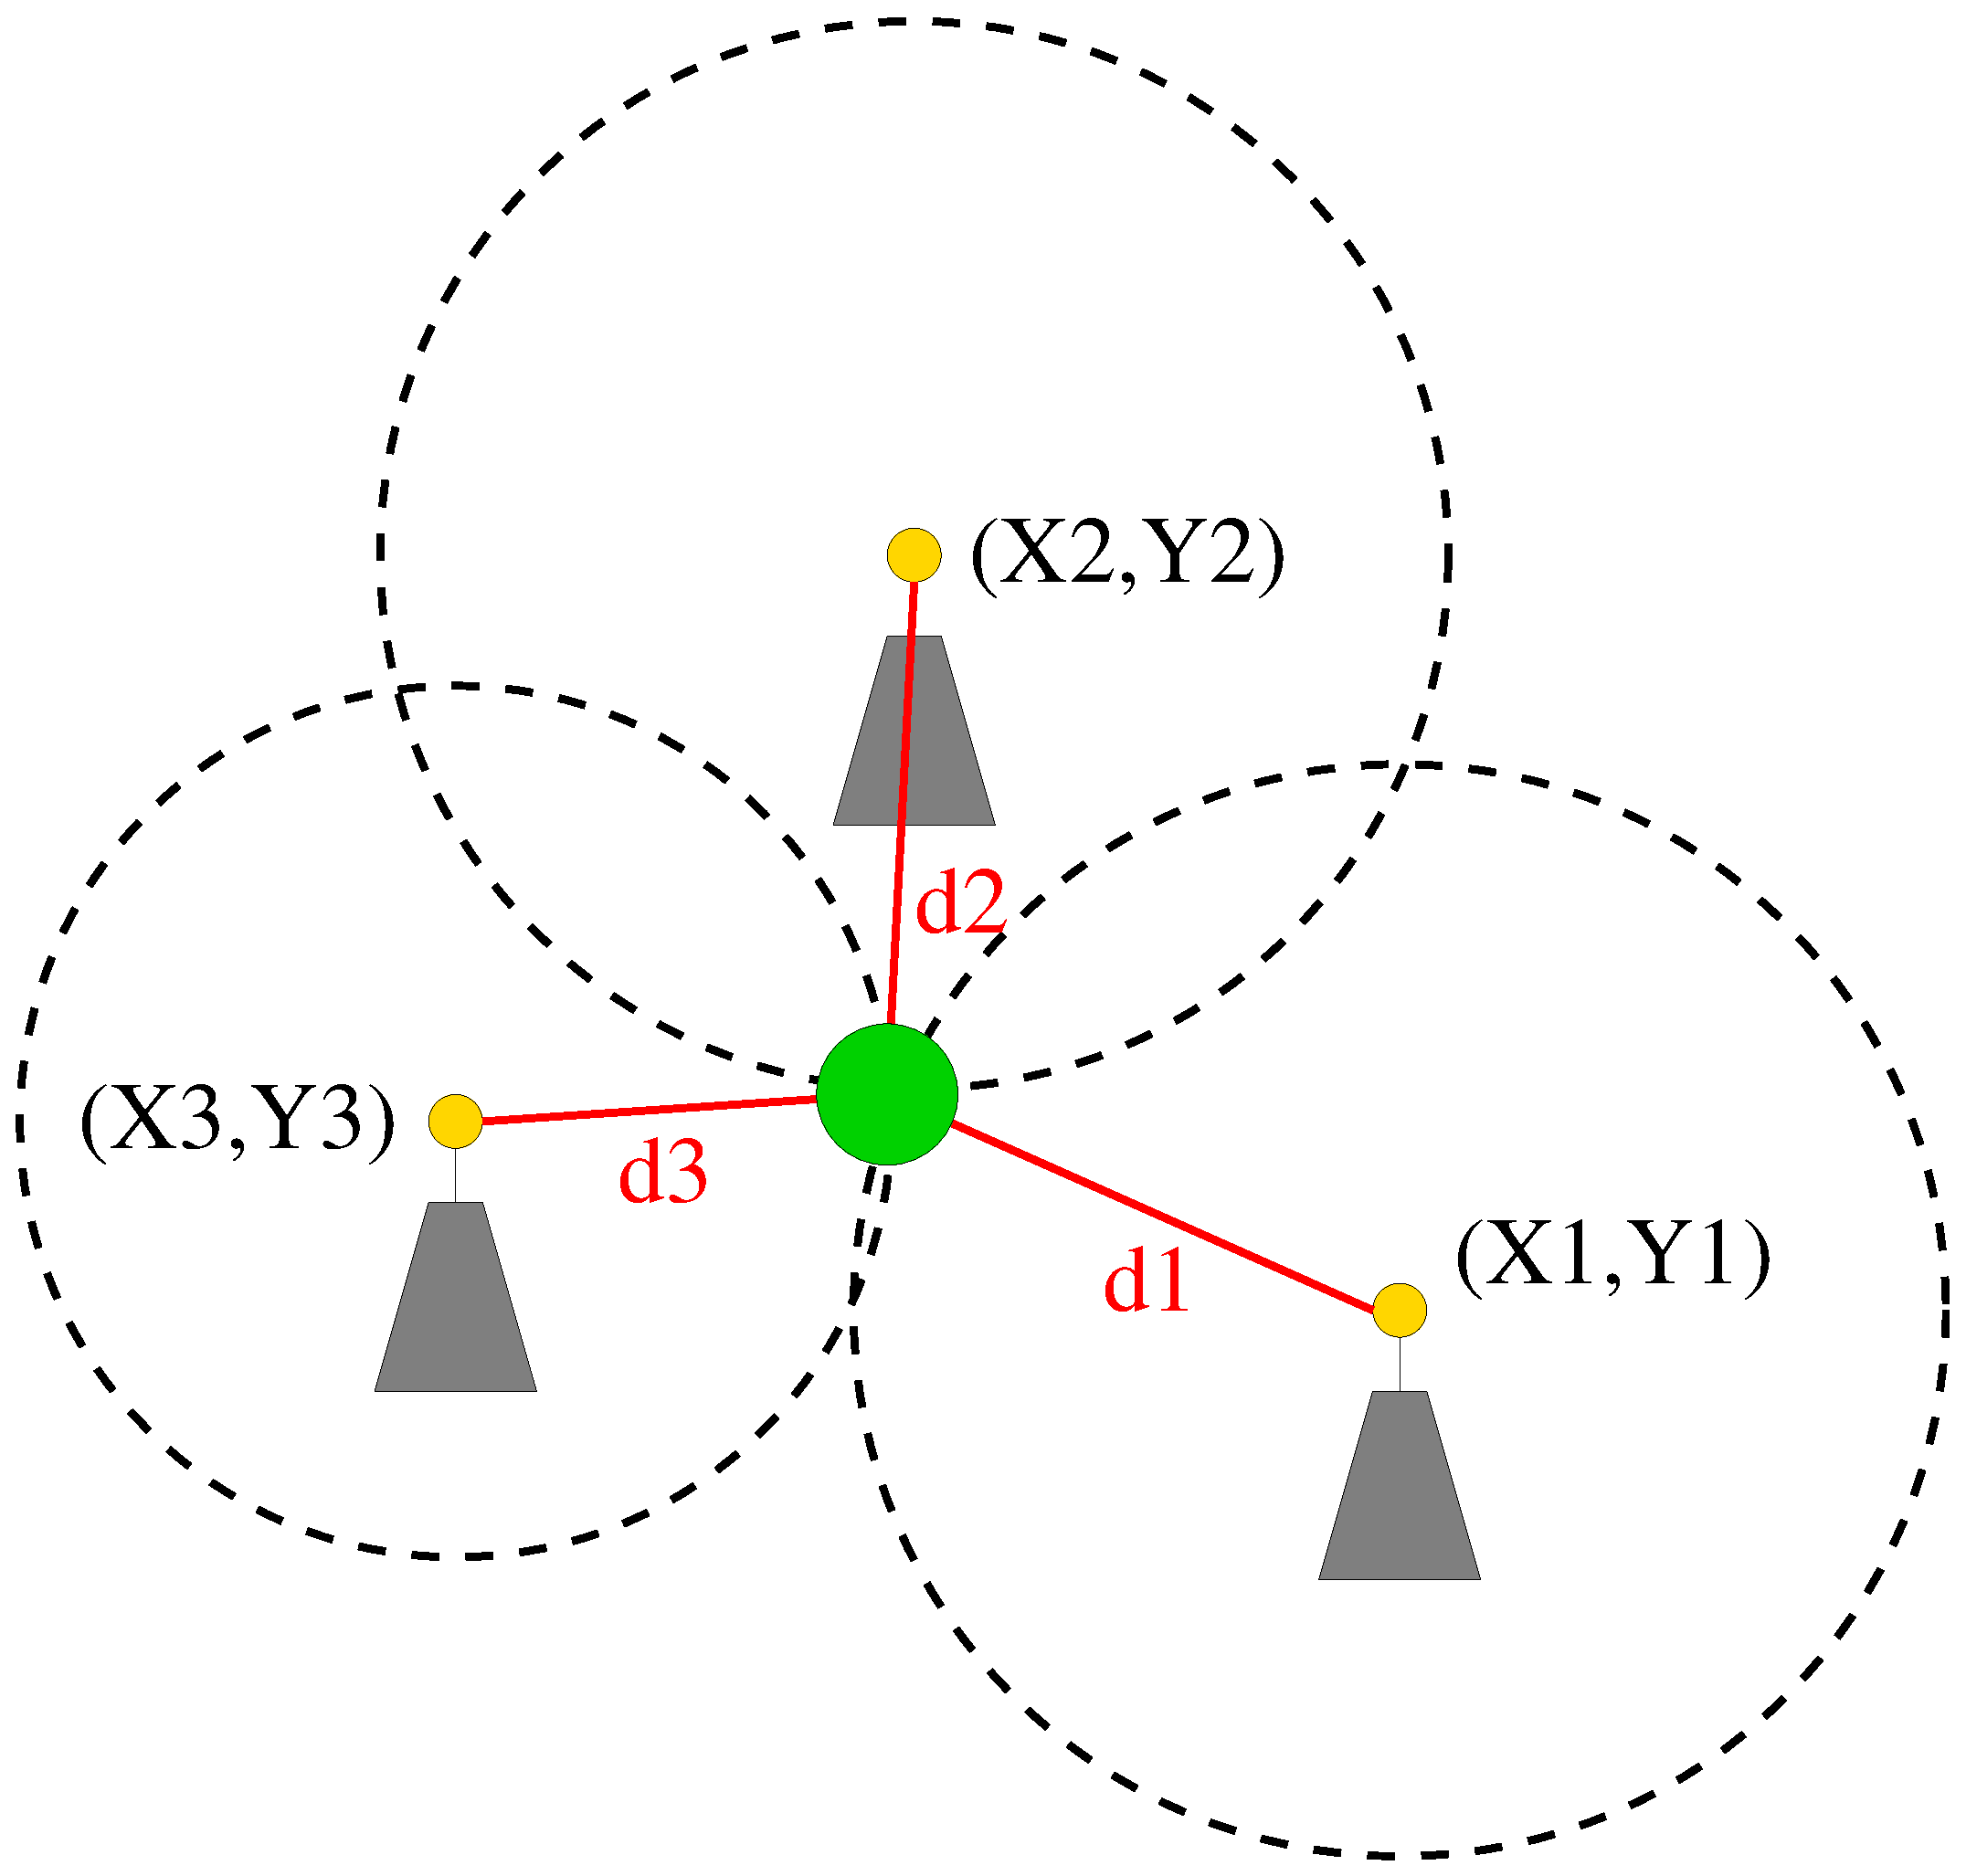
\includegraphics[width=0.7\linewidth]{figures/lateration.eps}
				\caption{\small Lateration example
				\label{fig:lateration}}
			\end{figure}%
% 			\begin{itemize}
% 				\item Also uses ranging techniques to add constraints.
% 			\end{itemize}

		\end{minipage}%
	}
	
	\frame{\frametitle{Range-free and Range-based}
		Range-free protocols:
		\begin{itemize}
 			\item Only consider the effective connection with surrounding Anchors.
 			\item Usually consume less battery.
 			\item Error is subject to the number of connections to different Anchors.
		\end{itemize}
		Range-based protocols:
		\begin{itemize}
			\item Use ranging techniques to restrict the underlying optimization problem.
			\item Increased battery consumption, usually subjected to the ranging technique used.
			\item The error is usually reduced due to the availability of more data.
		\end{itemize}

	}
	
\end{document}
